\section{Introduction}
\label{sec:intro}
Modern machine learning methods for semantic segmentation have shown excellent performances across numerous medical domains in recent years. These advances have been spearheaded by new deep learning based approaches that leverage large amounts of images and annotations. Unfortunately, it is well known that generating substantial quantities of segmentation annotations for medical imaging is extremely burdensome. This is in part due to the need for domain specific knowledge in clinical applications, but also due to the fact that many medical imaging modalities are inherently 3-dimensional (\eg CT, MRI, PET, OCT, etc.) or video based (\eg endoscopy, microscopy, etc. ). The latter point greatly increases the time and effort necessary to manually segment even just a few volumes or videos.

To overcome this important bottleneck, semi-supervised methods in medical imaging have been a core research focus. Sub-domains have included for example, active learning~\cite{sener18, KonSznFua15}, self-supervised methods~\cite{chen19, jamaludin17}, and crowd-sourcing based annotating~\cite{salvador13, heim18}: all of which have variants tailored for segmentation tasks. Broadly speaking, the core idea in each of these is to maximize the value of individual manually generated annotations for subsequent training of segmentation models.

In this context, the present work targets the problem of segmenting specific objects of interest in medical volumes or videos using sparse point-wise supervision. Specifically, point-wise supervision involves providing a single click per frame to denote the object of interest. As observed in~\cite{bearman16}, the advantage of point-wise supervision is that they are extremely easy to collect, reliable and efficient. While a manual segmentation will take 239 seconds on average for a single PASCAL VOC image, the corresponding multi-class point-wise annotations only requires 22 seconds on average. This speed gain comes at the cost of sparse annoations in contrast to full semantic segmentations. However, methods to generate full segmentations from these point-wise annotations have already shown promising performances in medical imaging~\cite{vilarino2007,ferreira12,khosravan16,lejeune17,lejeune18}, and the present work follows this specific line of research. 
%While some of these methods focused on designed methods tailored to specific applications or modalities~\cite{vilarino2007,khosravan16}, more recent methods have looked to tackle the problem for a broad range of imaging modalities and structures of interest~\cite{bearman16,lejeune17,lejeune18}.

Our goal is thus to generate a sequence of binary segmentation masks for an object of interest present in a volume or video using point-wise annotations in that specific volume (see Fig.~\ref{fig:intro}). The point-wise annotations can be provided by manual clicks~\cite{ferreira12,bearman16,lejeune18}, or using a gaze tracker~\cite{vilarino2007,khosravan16,lejeune17,lejeune18}, and always relate to a single object instance visible at all times. That is, the annotations only provide explicit information as to the location of the object of interest and no information regarding the background is known. In terms of learning, this implies that positive samples are given by the annotations (\ie locations on the object of interest throughout the data), while no explicit negative samples are available. Instead, a large unlabeled set of samples is accessible without knowing which of these is positive or negative. This problem setting is known as P(ositive)-U(nlabeled) learning~\cite{li03,li05,duplessis14,duplessis15} and lies at the heart of this work.

\begin{figure*}[t]
\centering
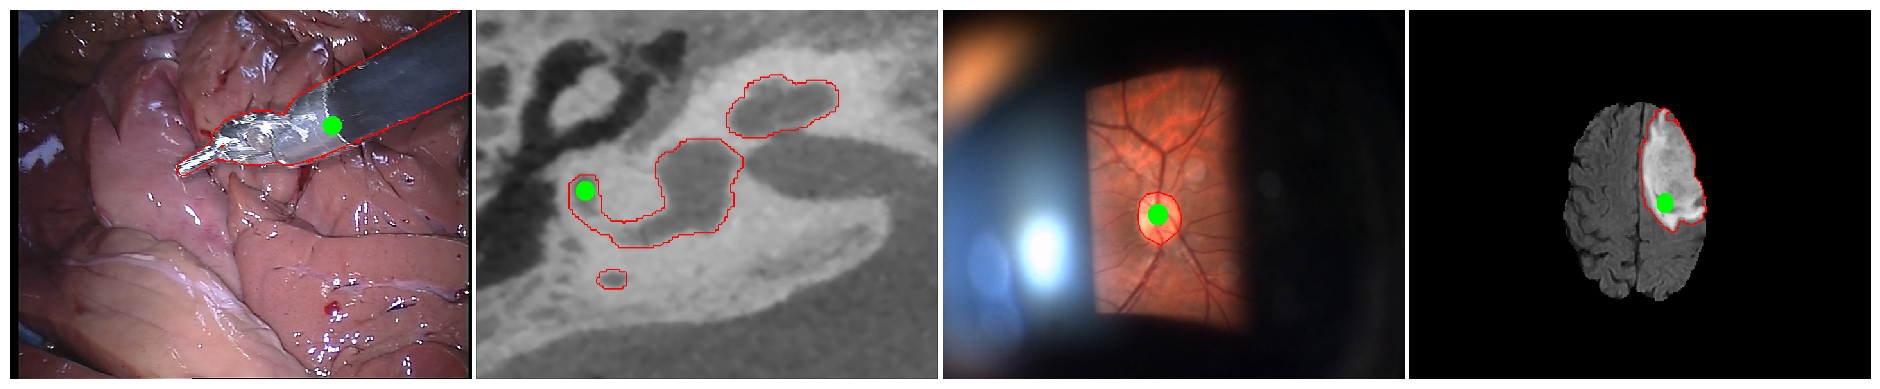
\includegraphics[width=0.99\textwidth]{intro.png}
\caption{Examples of image frames in different imaging modalities with different objects of interest to segment. In each example, a 2D point annotation is show in green and the complete pixel-wise groundtruth segmentation is shown in red. Applications shown are (from left to right): Video frame of a surgical instrument during minimally invasive surgery, a single slice from a CT scan depicting a human cochlea, video frame from a slitlamp examination of the optic nerve, brain slice from an MRI scan showing a tumor.}
\label{fig:intro}
\end{figure*}

Indeed, recent works in segmentation by point-wise annotations have cast their methods in such PU learning frameworks~\cite{bearman16,lejeune17,lejeune18}. In~\cite{lejeune17}, a modified exponential loss within a boosting framework was used to learn the object appearance model, whereas~\cite{lejeune18} used a bagging strategy inspired by random forests to do the same. Conversely,~\cite{bearman16} used object shape priors when training a Convolutional Neural Network (CNN) which worked well on large datasets, but poorly within a given volume or video sequence. Importantly however, the shape priors act as an important regularizer when training deep models in PU learning settings. This fact was reiterated in~\cite{kiryo17}, which proposed a non-negative unbiased risk estimator when training CNNs with PU settings. Unfortunately however, it heavily depends on knowing the proportion of positives in the data before hand and thus heavily restricts its applicability.

In this work, we introduce a novel PU learning method that allows for high segmentation performances from point-wise annotations. Our approach leverages the non-negative unbiased risk estimator of~\cite{kiryo17} to infer the likelihood of the object presence throughout the data. To do this, we introduce a self-supervised strategy to estimate the proportion of positive samples per frame using a recursive bayesian approach within our training procedure. Our method has the benefit of only needing a single upper-bound initialization value while allowing per-frame estimates to be computed.
We further combine the latter estimates with a multi-path tracking framework that explicitly leverages the spatio-temporal relations of over-segmented regions. This allows the output of our model to be regularized throughout the data volume.
We show experimentally that our pipeline brings important performance gains over state-of-the-art methods across a broad range of image modalities and object types.

%An annotator is given a video or volume that contains a single object of interest, and is asked to give a maximum of one click on each frame where the object lies.
%In \cite{lejeune18}, authors provide a general framework that builds up on multi-object tracking.
%In particular, the segmentation problem is formulated as a maximum a posteriori problem where the binary random variable to optimize for assign superpixels to the foreground or background.
%Through the Markov assumption, the problem is then cast into a network flow problem.
%The latter approach requires two kind of models to determine the costs associated to edges.
%(1) A foreground model, which gives the cost that a path would incur when transiting through a given superpixel, and (2) and transition model which gives the cost of passing from one superpixel to another located on a past or future frame.
%
%Despite the effectiveness of the latter approach, we note that component (1) requires to train an auto-encoder as a pretext task to obtain deep-features, which are then used by a simple bagging of decision trees applicable to PU learning to infer the foreground probabilities.
%First, as the late-stage bagging model considers all over-segmented regions as independent samples,
%the spatial configuration of the object of interest is not explicitly taken into account.
%Second, even though authors add an image-wise gaussian prior to the reconstruction error as an attempt to penalize errors around the object of interest,
%the loss function of the auto-encoder does not specifically target the task of segmentation.
%
%In the present work, we overcome the above limitations through the following contributions.
%\begin{itemize}
%    \item We take a more direct approach by leveraging the non-negative unbiased risk estimator of \cite{kiryo17}, which we use as a loss function of a Convolutional Neural Network to infer the foreground probabilities.
%  \item Furthermore, as the latter loss function requires accurate class-priors to be effective,
%    we devise a self-supervised strategy to estimate them through a recursive bayesian approach, initialized with a single upper-bound value.
%\end{itemize}

%%% Local Variables:
%%% mode: latex
%%% TeX-master: "main"
%%% End:
